\documentclass{beamer}
\mode<presentation>{\usetheme{default}}
\usecolortheme{dolphin}
\useoutertheme{split}
\usepackage{makecell}
\usepackage{ctex}
\usepackage{xcolor}
\usepackage{multirow}
\usepackage{array}
\usepackage{booktabs}
\usepackage{setspace}
\usepackage{graphics}
%\usefonttheme{professionalfonts}
%\usepackage{fontspec}

\title{编译实习课程改革}
\author{李汪洋\ 李佳蔚\ 梁家硕}
\date{}

\begin{document}

\frame{\titlepage}

\section{编译课程与改革}

\subsection{课程问题及解决方案}

\begin{frame}
    \frametitle{课程问题及解决方案}
    \begin{spacing}{1.3}
    \begin{table}
        \begin{tabular}{c|c}
            \hline \hline
            编译课程存在的问题 & 解决方案 \\
            \hline
            \makecell{对于中下游的同学任务量大\\对于能力比较强的同学任务轻松\\同学们对Java可能不熟悉} 
            & \makecell{MiniJava换成更简练的MiniC\\减少中间代码转换层数\\增设扩展内容\\对完成扩展的同学提供加分} \\
            \hline
            \makecell{实习课与原理课进度不协调\\期中前后任务量分配不合理}
            & 重新安排实习课程进度 \\
            \hline
            前一阶段的遗留问题影响之后进度
            & \makecell{任务模块化\\可提供前一阶段的标准模块} \\
            \hline \hline
        \end{tabular}
    \end{table}
    \end{spacing}
\end{frame}


\section{MiniC编译器}

\subsection{语言设计}

\begin{frame}
    \frametitle{MiniC $\cdot$ Eeyore $\cdot$ Tigger 语言设计}
    \begin{itemize}
        \setlength{\itemsep}{.5cm}
        \item MiniC是C语言的一个子集,对C语言进行了\textbf{大量}删减,易于实现。

        \item Eeyore /\texttt{'}\i:ju\textschwa(r)/ 是一种三地址码,由龙书上使用的三地址码扩展而来,用作MiniC分析程序的输出格式。

        \item Tigger /\texttt{'}t\i g\textschwa(r)/ 是对Eeyore进行寄存器分配后的输出格式,语法与Eeyore很像,面向RISC-V。
    
        \item Tigger与Eeyore两种中间表示的设计十分简洁,结构清晰,一看便懂,极大地降低同学们的学习成本。
    \end{itemize}
\end{frame}

\frame{
    \frametitle{Eeyore与Tigger命名}
    \begin{center}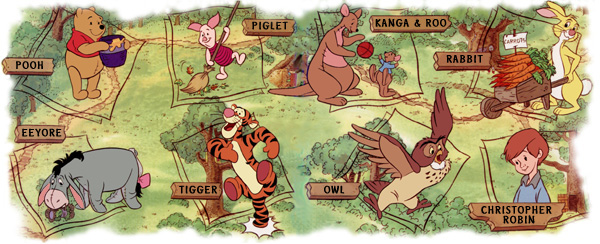
\includegraphics[width=10cm]{name}\end{center}
    Eeyore与Tigger继承了MiniJava编译器中使用的Piglet与Kanga两种中间表示的命名传统,取自同一动画 “winnie pooh”。
}

\subsection{改进}

\begin{frame}
    \frametitle{两处较大的改进}
    据调查,类型检查与寄存器分配是课程中最难的两部分,因此我们针对性地做了两处改进。
    \begin{itemize}
        \item MiniC的类型检查与MiniJava相比大大简化,只有int和一维int数组,减轻了同学们的任务量。
        \item 推荐采用Linear Scan寄存器分配算法,相较于图染色算法,实现难度大大降低,且实际效果不亚于图染色。
    \end{itemize}
\end{frame}

\subsection{进度安排}

\begin{frame}
    \frametitle{进度安排}
    我们根据自身完成MiniC编译器的经验,给未来的同学们作出如下进度安排:
    \begin{itemize}
        \item 第1--2周:努力学习编译原理,并预习语法制导翻译部分,并尝试学习安装riscv-gcc。

        \item 第3--7周:完成MiniC$\rightarrow$Eeyore。

        \item 第8--11周:完成Eeyore$\rightarrow$Tigger。

        \item 第12--13周:完成Tigger$\rightarrow$RISC-V。

        \item 第14周:编写实验报告。

        \item 考虑到同学们有期中期末考试以及假期,预留出了2周左右的时间。
    \end{itemize}
\end{frame}

\section{实例演示}

\frame{\centering \Huge 演示}

\section{完成情况}

\subsection{完成进度与分工}

\begin{frame}
    \frametitle{完成进度与分工}
    \begin{itemize}
        \item MiniC前端\qquad\qquad 期中前完成(梁家硕,李佳蔚)
        \item Eeyore模拟器\qquad\qquad 期中前完成,期中后优化(李汪洋)
        \item Tigger模拟器\qquad\qquad 第13周完成(梁家硕)
        \item MiniC,Eeyore,Tigger语法制定\qquad 学期从头到尾一直在修订
        \item 寄存器分配\qquad\qquad 第14--15周完成(李佳蔚)
        \item Tigger转RISC-V\qquad\qquad 第15周完成(李汪洋)
        \item MiniC测试程序与数据\qquad 第15周完成(梁家硕)
        \item 测试平台搭建\qquad\qquad 第15周完成(李汪洋)
    \end{itemize}
\end{frame}

\subsection{尚存的问题}

\begin{frame}
    \frametitle{尚存的问题}
    \begin{itemize}
        \setlength{\itemsep}{.5cm}
        \item 标准模块缺少兼容性测试
        \item 没有具体设置扩展内容
        \item 缺少教学实践检验
    \end{itemize}
\end{frame}

\end{document}
